\section{Wyniki regresji}
\label{sec:regression}

W rozdziale przedstawiono wyniki sześciu badań regresji, po trzy dla zbiorów \texttt{activation} i \texttt{cube}. Miarą jest MSE testowe w oryginalnej skali odpowiedzi, podawane jako mediana i kwartyle po $10$ ziarnach, osobno dla punktów w zakresie zbioru uczącego \eqref{eq:mse-inside} i poza nim \eqref{eq:mse-outside}. Błąd w zakresie mierzy dopasowanie do funkcji w obszarze danych uczących, a błąd poza zakresem zależy tylko od tego, jak sieć przedłuża swoją funkcję tam, gdzie nie widziała żadnych danych.

\subsection{Funkcje aktywacji}
\label{sec:regression-activations}

Wyniki badania funkcji aktywacji dla zbioru \texttt{activation} przedstawiono na Rysunku~\ref{fig:regression-activation-activations-heatmaps}. W zakresie zbioru uczącego najlepsza przy każdej liczności jest funkcja tanh, z medianą MSE od \num{0.0208} do \num{0.0372}. Funkcja sigmoidalna osiąga od \num{0.0319} do \num{0.156}, a ReLU i leaky ReLU od \num{0.269} do \num{2.63}. Poza zakresem różnice sięgają trzech rzędów wielkości. Mediana MSE wynosi od \num{0.600} do \num{2.33} dla funkcji tanh, od \num{38.0} do \num{120} dla funkcji sigmoidalnej i od \num{1410} do \num{2200} dla ReLU i leaky ReLU.

\begin{figure}[H]
    \centering
    \begin{subfigure}[b]{0.49\textwidth}
        \centering
        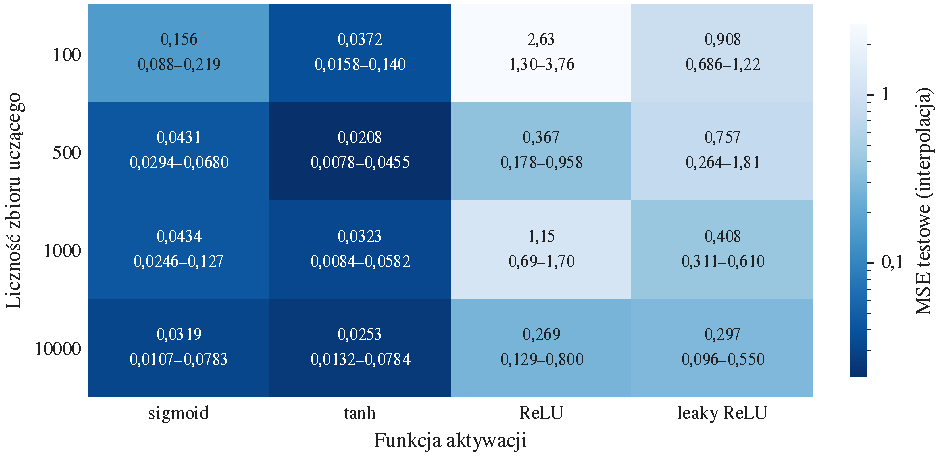
\includegraphics[width=\textwidth]{regression/activation-activations/results/heatmap_inside.pdf}
        \caption{w zakresie zbioru uczącego}
    \end{subfigure}
    \hfill
    \begin{subfigure}[b]{0.49\textwidth}
        \centering
        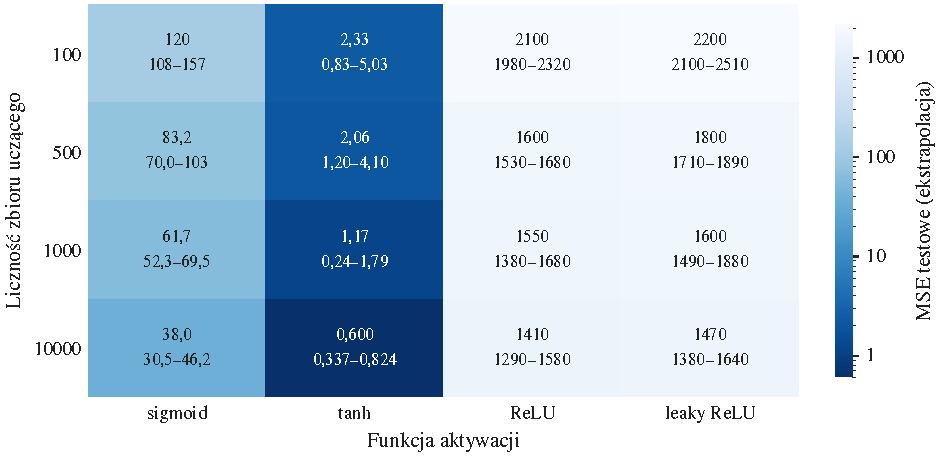
\includegraphics[width=\textwidth]{regression/activation-activations/results/heatmap_outside.pdf}
        \caption{poza zakresem zbioru uczącego}
    \end{subfigure}
    \caption{MSE testowe na zbiorze \texttt{activation} w zależności od funkcji aktywacji warstw ukrytych i liczności zbioru uczącego: mediana i kwartyle po $10$ ziarnach.}
    \label{fig:regression-activation-activations-heatmaps}
\end{figure}

Źródło tych różnic widać na Rysunku~\ref{fig:regression-activation-activations-gallery}, który dla każdej funkcji aktywacji pokazuje jedno z $10$ uczeń przy liczności \num{1000}: to, którego MSE testowe jest najbliższe medianie po ziarnach. W zakresie danych uczących wszystkie cztery sieci pokrywają się z funkcją docelową. Poza nim sieci z funkcjami tanh i sigmoidalną nasycają się tak jak funkcja docelowa, przy czym sieć z funkcją sigmoidalną na lewym krańcu dochodzi do innego poziomu. Sieci z ReLU i leaky ReLU przedłużają funkcję prostą, która coraz bardziej oddala się od nasyconej funkcji docelowej.

\begin{figure}[H]
    \centering
    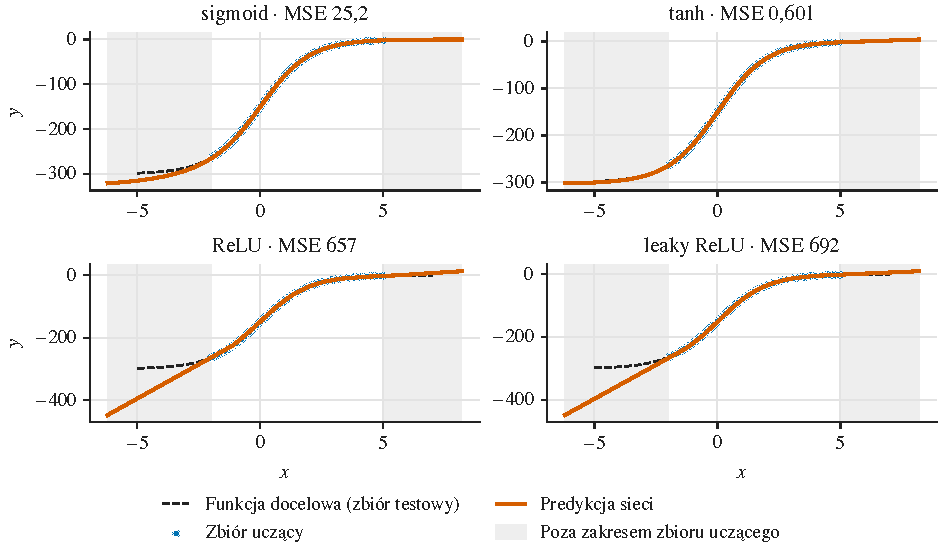
\includegraphics[width=0.9\textwidth]{regression/activation-activations/results/gallery_1000.pdf}
    \caption{Funkcja sieci na zbiorze \texttt{activation} przy liczności \num{1000} dla każdej funkcji aktywacji: uczenie o MSE testowym najbliższym medianie po ziarnach i jego MSE testowe. Szare pasy oznaczają obszar poza zakresem zbioru uczącego.}
    \label{fig:regression-activation-activations-gallery}
\end{figure}

Daleko od danych pobudzenia neuronów pierwszej warstwy ukrytej rosną co do wartości bezwzględnej liniowo z $x$. Funkcje tanh i sigmoidalna mają ograniczony zbiór wartości (Tabela~\ref{tab:activations}), więc ich wyjścia stają się stałe, a z nimi cała funkcja sieci. Sieć z funkcjami ReLU lub leaky ReLU jest funkcją kawałkami liniową, więc daleko od danych jest liniowa \cite{xu2021}. Funkcja docelowa zbioru \texttt{activation} nasyca się na obu krańcach (podrozdział~\ref{sec:problem-datasets}), dlatego przedłużenie stałe pasuje do niej, a przedłużenie liniowe nie.

Wyniki dla zbioru \texttt{cube} przedstawiono na Rysunku~\ref{fig:regression-cube-activations-heatmaps}. W zakresie zbioru uczącego przy liczności \num{100} najlepsza jest funkcja tanh (\num{0.680}), a najsłabsza funkcja sigmoidalna (\num{5.94}). Przy liczności \num{10000} kolejność się zmienia: funkcja sigmoidalna osiąga \num{0.196}, tanh \num{0.266}, a ReLU i leaky ReLU \num{0.463} i \num{0.753}. Poza zakresem wszystkie sieci mają błędy rzędu $10^{4}$--$10^{5}$. Najmniejsze ma leaky ReLU (od \num{62200} do \num{75700}), następnie ReLU (od \num{73100} do \num{82600}), tanh (od \num{83400} do \num{94500}) i funkcja sigmoidalna (od \num{89100} do \num{121000}).

\begin{figure}[H]
    \centering
    \begin{subfigure}[b]{0.49\textwidth}
        \centering
        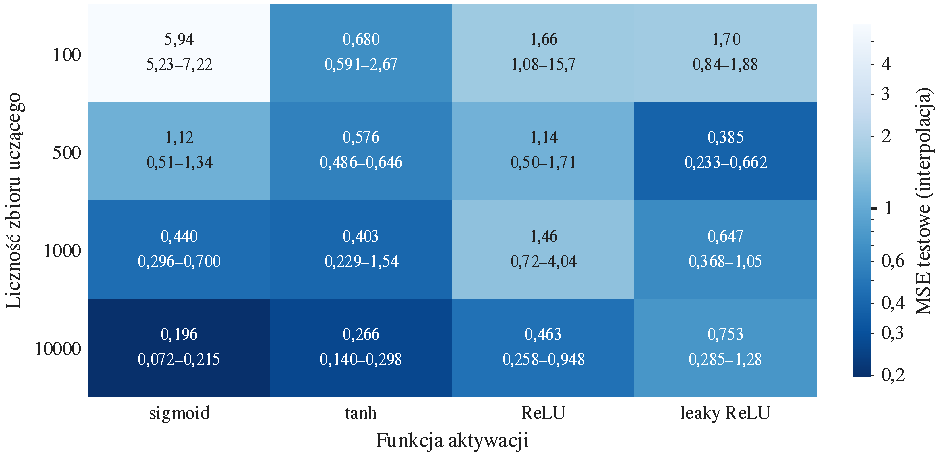
\includegraphics[width=\textwidth]{regression/cube-activations/results/heatmap_inside.pdf}
        \caption{w zakresie zbioru uczącego}
    \end{subfigure}
    \hfill
    \begin{subfigure}[b]{0.49\textwidth}
        \centering
        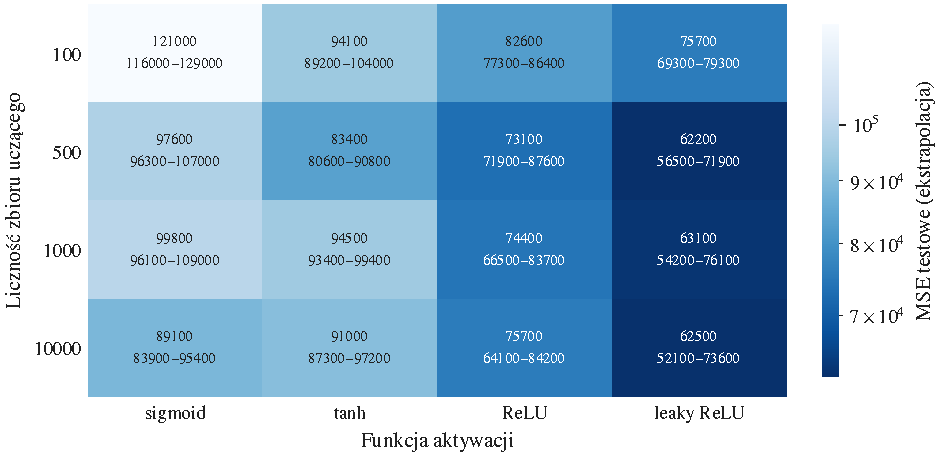
\includegraphics[width=\textwidth]{regression/cube-activations/results/heatmap_outside.pdf}
        \caption{poza zakresem zbioru uczącego}
    \end{subfigure}
    \caption{MSE testowe na zbiorze \texttt{cube} w zależności od funkcji aktywacji warstw ukrytych i liczności zbioru uczącego: mediana i kwartyle po $10$ ziarnach.}
    \label{fig:regression-cube-activations-heatmaps}
\end{figure}

Funkcja docelowa zbioru \texttt{cube} na krańcach szybko rośnie co do wartości bezwzględnej, szybciej niż jakakolwiek prosta. Żadna z badanych sieci nie może więc jej przedłużyć, a ranking poza zakresem mówi tylko, której sieci przedłużenie najmniej odbiega od funkcji docelowej. Przedłużenie liniowe sieci z ReLU i leaky ReLU podąża za wzrostem funkcji dłużej niż przedłużenie stałe sieci z funkcjami tanh i sigmoidalną.

\subsection{Architektura sieci}
\label{sec:regression-architectures}

Wyniki badania architektur dla zbioru \texttt{activation} przedstawiono na Rysunku~\ref{fig:regression-activation-architectures-heatmaps}. Sieć bez warstw ukrytych, czyli model liniowy, ma w zakresie zbioru uczącego medianę MSE od \num{693} do \num{708}. Sieci z warstwami ukrytymi osiągają od \num{0.00225} do \num{0.470}, czyli co najmniej o trzy rzędy wielkości mniej. Ich kolejność zmienia się z licznością, a kwartyle są szerokie, więc nie wskazują jednej najlepszej architektury. Poza zakresem sieci z jedną warstwą ukrytą mają medianę MSE od \num{4.55} do \num{54.4}, a sieci z co najmniej dwiema warstwami od \num{0.492} do \num{10.3}. U sieci 64-64 i 64-64-64-64 mediana mieści się przy każdej liczności w przedziale od \num{0.984} do \num{1.77}. Największe błędy wśród sieci z warstwami ukrytymi ma jedna warstwa z $64$ neuronami, od \num{18.9} do \num{54.4}. Sieć bez warstw ukrytych ma poza zakresem ponad \num{3900}.

\begin{figure}[H]
    \centering
    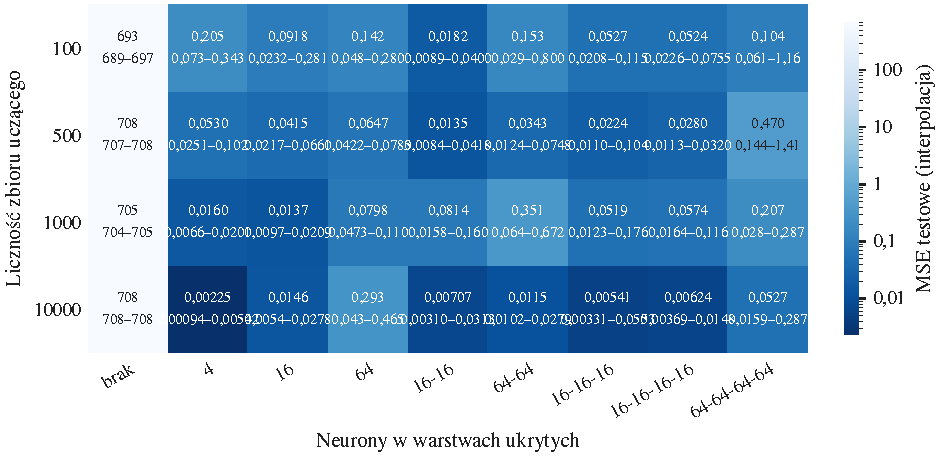
\includegraphics[width=\textwidth]{regression/activation-architectures/results/heatmap_inside.pdf}

    \vspace{1ex}
    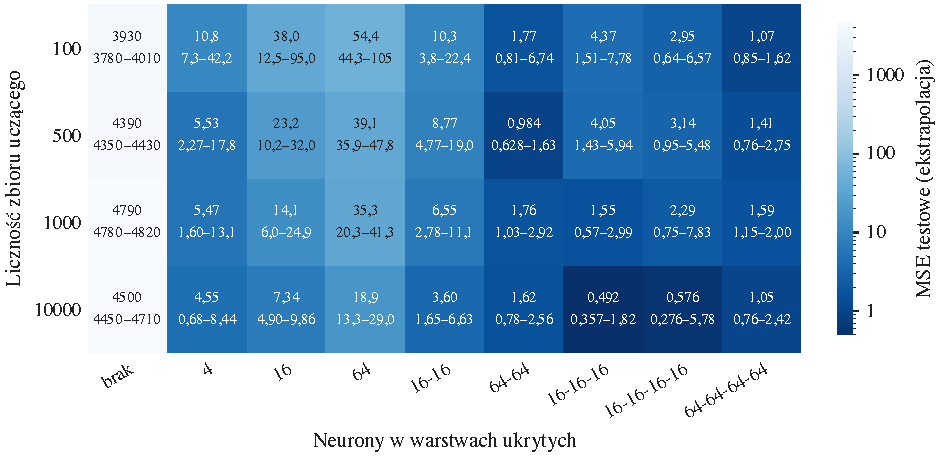
\includegraphics[width=\textwidth]{regression/activation-architectures/results/heatmap_outside.pdf}
    \caption{MSE testowe na zbiorze \texttt{activation} w zależności od architektury i liczności zbioru uczącego: mediana i kwartyle po $10$ ziarnach. Górny wykres: w zakresie zbioru uczącego. Dolny wykres: poza zakresem zbioru uczącego.}
    \label{fig:regression-activation-architectures-heatmaps}
\end{figure}

Wyniki dla zbioru \texttt{cube} przedstawiono na Rysunku~\ref{fig:regression-cube-architectures-heatmaps}. Model liniowy ma w zakresie zbioru uczącego medianę MSE od \num{889} do \num{1010}. Przy każdej liczności każda sieć z co najmniej dwiema warstwami ukrytymi jest lepsza od każdej sieci z jedną warstwą. Przy liczności \num{100} mediany wynoszą od \num{0.930} do \num{1.96} wobec od \num{11.6} do \num{30.9}, a przy liczności \num{10000} od \num{0.115} do \num{0.772} wobec od \num{1.12} do \num{1.49}. Poza zakresem najmniejszy błąd ma jedna warstwa z $64$ neuronami (od \num{59800} do \num{90400}), a największy spośród sieci z warstwami ukrytymi sieć 64-64-64-64 (od \num{137000} do \num{161000}).

\begin{figure}[H]
    \centering
    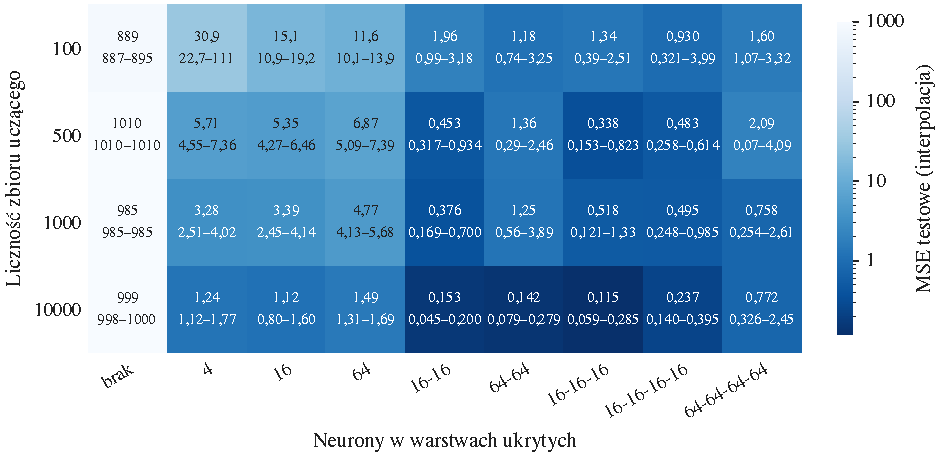
\includegraphics[width=\textwidth]{regression/cube-architectures/results/heatmap_inside.pdf}

    \vspace{1ex}
    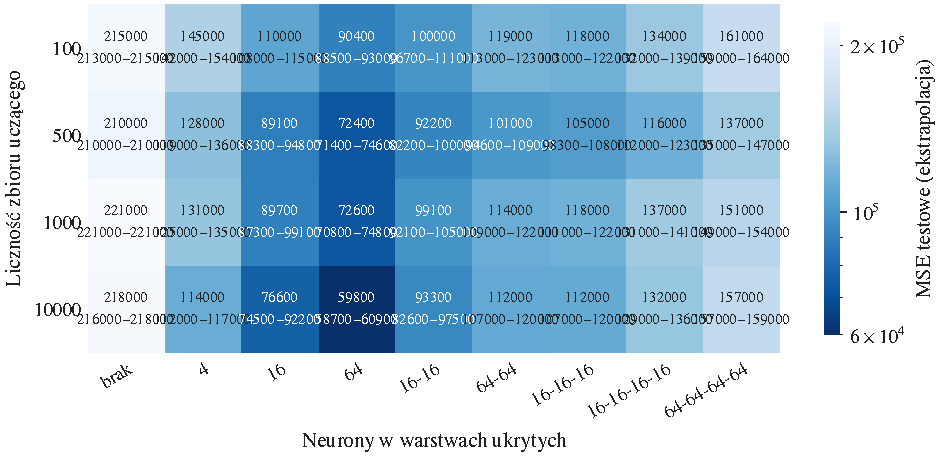
\includegraphics[width=\textwidth]{regression/cube-architectures/results/heatmap_outside.pdf}
    \caption{MSE testowe na zbiorze \texttt{cube} w zależności od architektury i liczności zbioru uczącego: mediana i kwartyle po $10$ ziarnach. Górny wykres: w zakresie zbioru uczącego. Dolny wykres: poza zakresem zbioru uczącego.}
    \label{fig:regression-cube-architectures-heatmaps}
\end{figure}

Funkcje sieci o różnych architekturach przy liczności \num{1000} pokazano na Rysunku~\ref{fig:regression-cube-architectures-gallery}, w tej samej postaci co na Rysunku~\ref{fig:regression-activation-activations-gallery}. Model liniowy nie dopasowuje się do funkcji nawet w zakresie danych uczących. Pozostałe sieci pokrywają się z funkcją docelową w zakresie danych, a poza nim wypłaszczają się, podczas gdy funkcja docelowa rośnie dalej. Sieci głębokie wypłaszczają się najszybciej, a sieć z jedną warstwą $64$ neuronów przedłuża wzrost najdłużej, stąd jej najmniejszy błąd poza zakresem.

\begin{figure}[H]
    \centering
    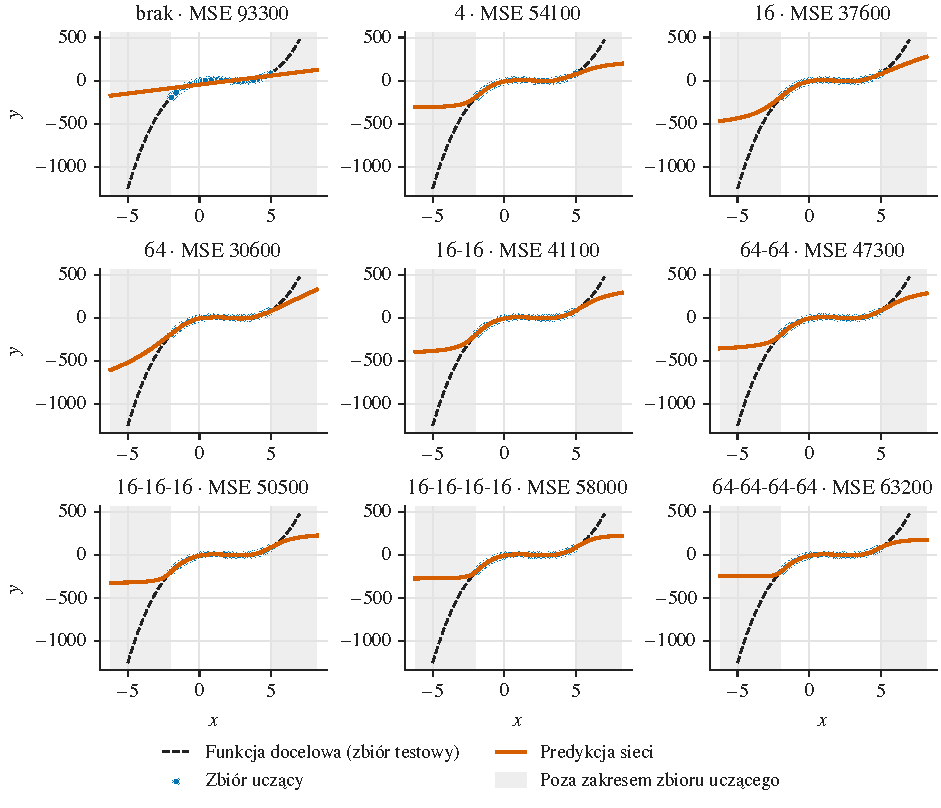
\includegraphics[width=0.9\textwidth]{regression/cube-architectures/results/gallery_1000.pdf}
    \caption{Funkcja sieci na zbiorze \texttt{cube} przy liczności \num{1000} dla każdej architektury: uczenie o MSE testowym najbliższym medianie po ziarnach i jego MSE testowe. Szare pasy oznaczają obszar poza zakresem zbioru uczącego.}
    \label{fig:regression-cube-architectures-gallery}
\end{figure}

\subsection{Funkcje straty}
\label{sec:regression-losses}

Wyniki badania funkcji straty przedstawiono na Rysunkach~\ref{fig:regression-activation-losses-heatmaps} i~\ref{fig:regression-cube-losses-heatmaps}. Sieć uczona na MSE jest w zakresie zbioru uczącego wyraźnie lepsza od sieci uczonej na MAE. Mediana MSE sieci uczonej na MAE jest od \num{14.6} do \num{22.6} razy większa w zbiorze \texttt{activation} i od \num{5.91} do \num{8.21} razy większa w zbiorze \texttt{cube}. Poza zakresem sieć uczona na MSE jest lepsza w zbiorze \texttt{activation} (od \num{2.81} do \num{5.66} razy), a w zbiorze \texttt{cube} stosunek median wynosi od \num{0.93} do \num{1.10}, więc nie ma systematycznej różnicy.

\begin{figure}[H]
    \centering
    \begin{subfigure}[b]{0.49\textwidth}
        \centering
        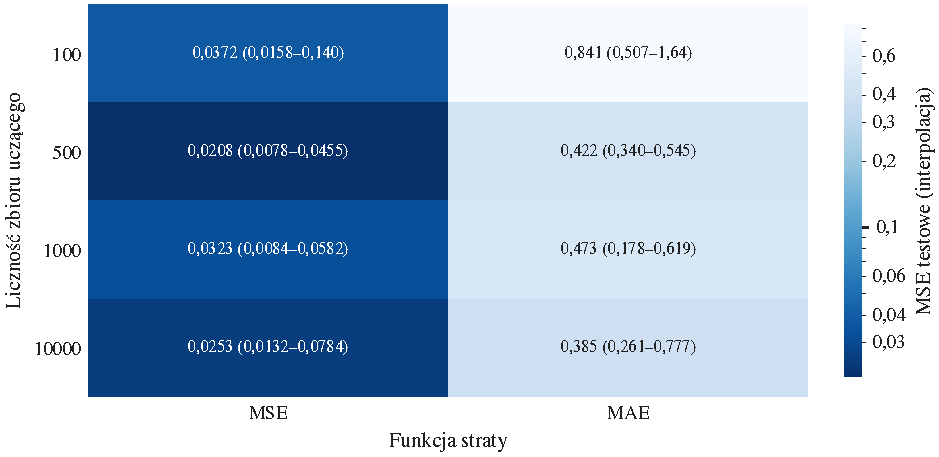
\includegraphics[width=\textwidth]{regression/activation-losses/results/heatmap_inside.pdf}
        \caption{w zakresie zbioru uczącego}
    \end{subfigure}
    \hfill
    \begin{subfigure}[b]{0.49\textwidth}
        \centering
        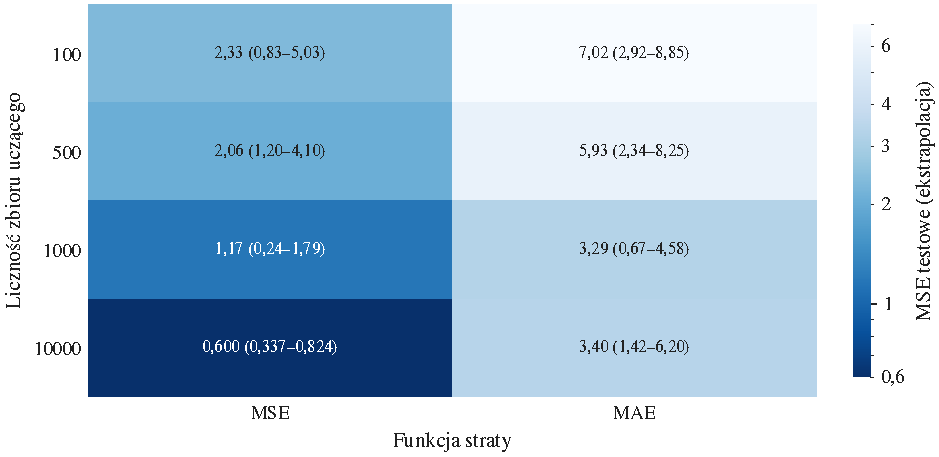
\includegraphics[width=\textwidth]{regression/activation-losses/results/heatmap_outside.pdf}
        \caption{poza zakresem zbioru uczącego}
    \end{subfigure}
    \caption{MSE testowe na zbiorze \texttt{activation} w zależności od funkcji straty i liczności zbioru uczącego: mediana i kwartyle po $10$ ziarnach.}
    \label{fig:regression-activation-losses-heatmaps}
\end{figure}

\begin{figure}[H]
    \centering
    \begin{subfigure}[b]{0.49\textwidth}
        \centering
        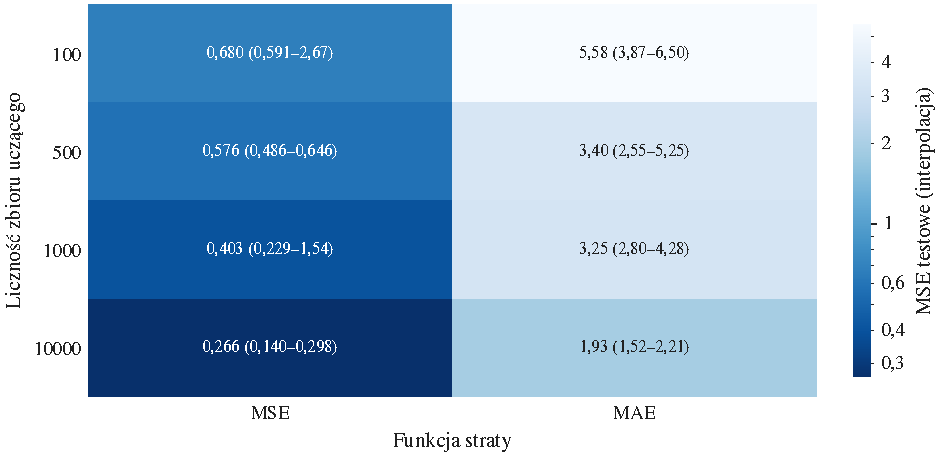
\includegraphics[width=\textwidth]{regression/cube-losses/results/heatmap_inside.pdf}
        \caption{w zakresie zbioru uczącego}
    \end{subfigure}
    \hfill
    \begin{subfigure}[b]{0.49\textwidth}
        \centering
        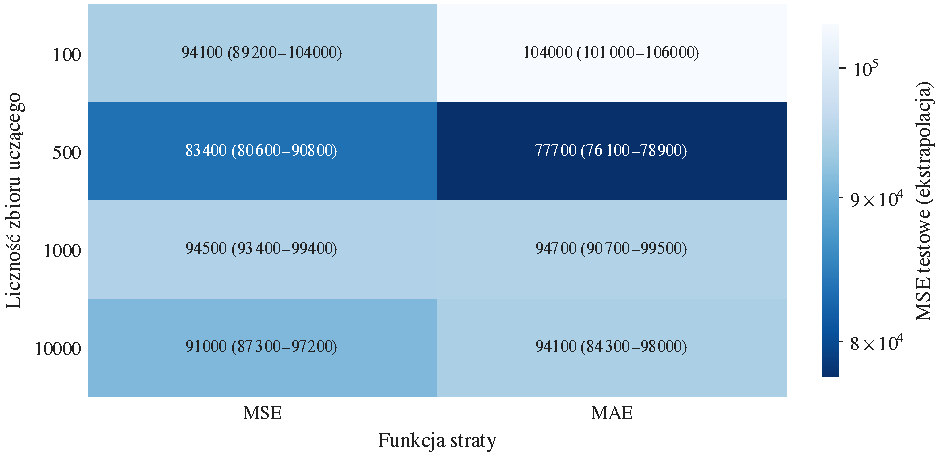
\includegraphics[width=\textwidth]{regression/cube-losses/results/heatmap_outside.pdf}
        \caption{poza zakresem zbioru uczącego}
    \end{subfigure}
    \caption{MSE testowe na zbiorze \texttt{cube} w zależności od funkcji straty i liczności zbioru uczącego: mediana i kwartyle po $10$ ziarnach.}
    \label{fig:regression-cube-losses-heatmaps}
\end{figure}

Miara MSE z definicji sprzyja sieci, która ją minimalizuje. Dlatego porównano też średni błąd bezwzględny na całym zbiorze testowym. W zbiorze \texttt{activation} sieć uczona na MSE jest lepsza także w tej mierze, z medianą od \num{0.374} do \num{0.619} wobec od \num{0.763} do \num{1.27} dla sieci uczonej na MAE. W zbiorze \texttt{cube} błąd bezwzględny na całym zbiorze testowym zależy głównie od punktów poza zakresem, a mediany obu sieci różnią się o co najwyżej \qty{8}{\percent}.

Sieć uczona na MAE ma również większe MSE na zbiorze uczącym, od \num{14.3} do \num{21.6} razy w zbiorze \texttt{activation} i od \num{7.08} do \num{8.30} razy w zbiorze \texttt{cube}. Gorszy wynik w zakresie danych wynika więc z mniej dokładnego dopasowania do zbioru uczącego, a nie z gorszego uogólniania. Zaletą MAE jest mniejsza wrażliwość na pojedyncze duże błędy, np. punkty odstające \cite[rozdz.~1.5.5]{bishop2006}. W badanych zbiorach punkty uczące leżą blisko funkcji docelowej (podrozdział~\ref{sec:problem-datasets}), więc ta zaleta nie ma okazji się ujawnić.
